\documentclass[../thesis.tex]{subfiles}

\begin{document}

\section{Collision statistics\label{sec:col}}
The results of several numerical tests and simulations are presented in this section. At first, the focus is on the current implementation of HDNS with lubrication effects taken into account. The results present the collision statistics of aerodynamically interacting droplets under one-way momentum coupling, i.e.\ the background flow does not feel the droplets. Next, the results of several computational tests on this implementation is provided, examining the impact of different physical as well as numerical parameters on the performance of the algorithm. Finally, the influence of considering two-way momentum coupling on the collision statistics of aerodynamically non-interacting droplets---that only interact with the background flow but do not feel each other (DNS)---is presented. Each subsection is finished with a summary of the key conclusions drawn from the results.



\subsection{Collision statistics of interacting droplets considering lubrication effects under one-way momentum coupling\label{sec:lub}}
The influence of considering lubrication forces in the AI of droplets will be discussed here. After a description of statistics of the background flow developed for this case, the dependence of the current HDNS implementation to both the time step size and the size of short-range interaction region (matching point) is analyzed to find the optimal values for each. Then, the effect of AI is investigated by comparing simulations conducted with and without lubrication effects as well as those when AI is not considered at all. In addition, the impact of important physical parameters, such as mass loading of water droplets, is investigated.



\subsubsection{Flow statistics}

\begin{table}[!b]%---------- T A B L E ----------
\center
  \begin{tabular}{ccccccc}
  \hline\hline
  $N$ & $\Delta t$ & $\nu$ & $\tau_\text{K}$ & $\eta_\text{K}$ & $T_e$ & $L_f$\\
  64 & 0.0042 & 0.0067 & 0.19 & 0.0036 & 3.86 & 1.62\\\hline
  $\epsilon$ & $u'$ & $R_{\lambda}$ & \textit{CFL} & $k_\text{max}\eta_\text{K}$ & $\mathcal{S}$ & $\mathcal{F}$\\
  0.18 & 0.82 & 76.86 & 0.23 & 1.1 & -0.42 & 4.51\\
  \hline\hline
  \end{tabular}
  \caption{Input parameter settings and average flow statistics in spectral units.}
  \label{tab:1}
\end{table}%------------------------------------

To examine lubrication effects, the computational grids are limited to $64^3$ nodes since the main focus is on the effect of aerodynamic interaction rather than the Reynolds number. The same flow field has been used in all the simulations in this subsection (\ref{sec:lub}). Before adding the particles to the domain, the flow field has evolved so as to reach a statistically stationary stage where the averages in flow statistics remain constant. The basic parameters and time-averaged statistics of the flow are listed in Table \ref{tab:1}, in which $N$ is the number of grid points---resolution---in each spatial direction, $\Delta t$ is the spectral time step chosen to evolve the flow, $\nu$ is the kinematic viscosity of the turbulent air given in spectral units, $\tau_\text{K}$ and $\eta_\text{K}$ are the Kolmogorov time and length scales, $T_e$ is the large-eddy turnover time, $L_f$ is the integral length scale, $\epsilon$ is the dissipation rate of turbulent kinetic energy, $u'$ is the r.m.s.\ of the fluctuations in velocity, $R_\lambda$ is the Taylor-microscale flow Reynolds number, \textit{CFL} is the Courant--Friedrichs--Lewy number, and $k_\text{max}\eta_\text{K}$ is the commonly defined resolution parameter which must be larger than unity. Furthermore, $\mathcal{S}$ and $\mathcal{F}$ are the skewness and flatness of longitudinal velocity gradient.



\subsubsection{Dependence of statistics to the time step size}
Including the lubrication forces into the model has a direct impact on the numerical properties, e.g.\ stability of integration, of the ordinary differential equations for tracking particles: Equations (\ref{eq:3}) and (\ref{eq:4}). Due to strong nonlinearity of these short-range aerodynamical forces, the resulting set of governing equations is stiff. As such, to guarantee the numerical stability, the integration scheme has to be properly adjusted. The time step size is of special importance in this regard and hence must be carefully optimized. If $\Delta t$ is too large, the algorithm may be unstable. Moreover, some collision statistics, for example the collision kernels, may be overestimated. This is because for a large $\Delta t$ the lubrication forces are sampled with an excessively coarse spatial resolution. On the other hand, if $\Delta t$ is very small the numerical cost of computations will be needlessly large. Therefore, to examine this problem, a number of simulations have been performed to find an optimal $\Delta t$. The largest time step, $\Delta t_\text{max}=4.24\times10^{-4}$~s, is the same as the one used to evolve the turbulent flow without particles, i.e.\ the spectral $\Delta t$ in Table \ref{tab:1}. Then, in subsequent simulations, the time step was consistently reduced by half up to $\Delta t_\text{max}/32$. It should be added that the total simulation time, roughly $100T_e$, was the same in all modeled cases.

The numerical experiments were divided into two groups. The first set of simulations was performed for droplets of relatively low inertia. In these simulations the Stokes number, defined as $St\equiv\tau_\text{p}/ \tau_\text{K}$, did not exceed $St = 0.36$. For such systems the effects of gravitational settling can be safely neglected. On the other hand, by referring to some former studies, e.g.\ \citet{HJ70} and \citet{RWMG11}, it is expected that the effect of lubrication forces is important. The droplet inertia was set by changing the value of energy dissipation rate. The droplet radii were fixed to $a_\text{p} = 40~\mu$m. In the second group of simulations we considered several different sizes of particles at fixed energy dissipation rate equal to $\epsilon = 400~\mathrm{cm^2/s^3}$. This setting is representative of moderate to strong convection in a cloud. For such systems gravity is important, hence the simulations were performed for both settling droplets and without gravity.   

\begin{figure}%---------- F I G U R E --------
\center
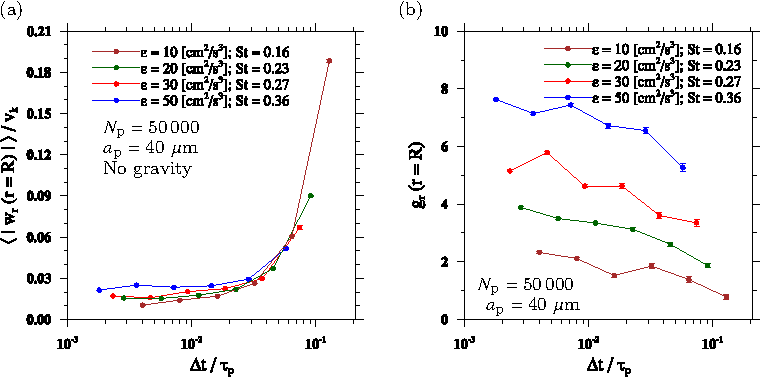
\includegraphics[width=\textwidth]{../figs/JFM/fig2.pdf}
\caption{Two-point collision statistics at contact computed using different time steps: (a) normalized radial relative velocity and (b) radial distribution function.}
\label{Fig2}
\end{figure}%------------------------------------

The effect of the time step size is assessed by comparing two-point collision statistics of \emph{almost touching} water droplets. Figure~\ref{Fig2}(a) shows the RRV normalized by the Kolmogorov velocity scale, computed in simulations with different $\Delta t$, which are normalized by the particle inertial response time. Corresponding values of the RDF are presented in Figure~\ref{Fig2}(b). In all these simulations the lubrication forces were considered. The main conclusion resulting from these simulations is that the statistics do not change much for $\Delta t < 0.04 \tau_\text{p}$. This seems to be a tradeoff between accuracy and numerical complexity.

The increase of the RRV at larger $\Delta t$ is a consequence of not sufficient representation of the short-range aerodynamic interaction. It should be recalled that the lubrication forces not only prevent collisions of approaching particles, but also restrain the pairs from receding from each other. This reversibility is an intrinsic feature of the solutions to the Stokes flow. As a result, the relative motion of the interacting droplets is more strongly correlated. In other words, the lubrication forces act similar to a hydraulic shock absorber and hence their effect must be thought of as that of a viscous damper, rather than a spring, in a simplified mass--spring--damper model. This can be readily confirmed by taking a look at Equation (\ref{eq:8}) in which the drag coefficients are multiplied by the velocities. This is a general feature of aerodynamic interaction forces, but in the case of lubrication forces this barrier is harder for particles to break through or escape from.

\begin{figure}%----------- F I G U R E ----------
\center
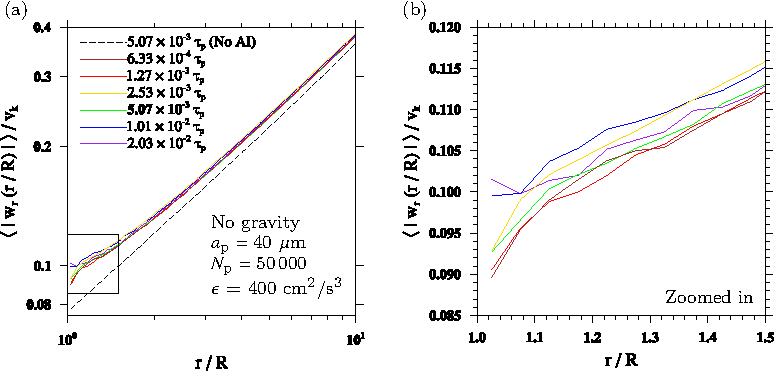
\includegraphics[width=\textwidth]{../figs/JFM/fig3.pdf}
\caption{Radial relative velocity computed using different time step sizes
for the normalized separation distance in the range (a) $1 < r/R < 10$ and (b) $1 < r/R < 1.5$
 with the set of droplets $a_\mathrm{p} = 40~\mathrm{\mu m}$ and $N_\mathrm{p} = 50\,000$.
The black rectangle in (a) marks the region that is enlarged and shown in (b).}
\label{Fig3}
\end{figure}%------------------------------------

The core results analyzed in the present study were computed assuming the energy dissipation rate $\epsilon = 400~\mathrm{cm^2/s^3}$. Therefore, the sensitivity of these simulations to the time step is analyzed more deeply. First, in Figure~\ref{Fig3}(a) we compare kinematic collision statistics computed in simulations without gravity at different separation ranges. As expected, for larger separation distances the RRV is not sensitive to the time step size. This can be explained by the fact that the lubrication forces are effective only at short ranges (see Figure~\ref{Fig1}). In turn, at near-contact separation distances, $1<r/R<1.5$, some minor changes in the RRV can be noticed. Accordingly, this region is enlarged and displayed in Figure~\ref{Fig3}(b). The data show slightly lower relative velocities for smaller time steps. This effect stems from the improvement in capturing short-range forces, which tend to decrease the magnitude---whether positive or negative---of the relative velocities between particles. The smaller the time step size, the more accurate the representation of the lubrication forces. Interestingly, for $\Delta t < 5.07 \times 10^{-3} \tau_\text{p}$ the differences are relatively low.

\begin{figure}%----------- F I G U R E ----------
\center
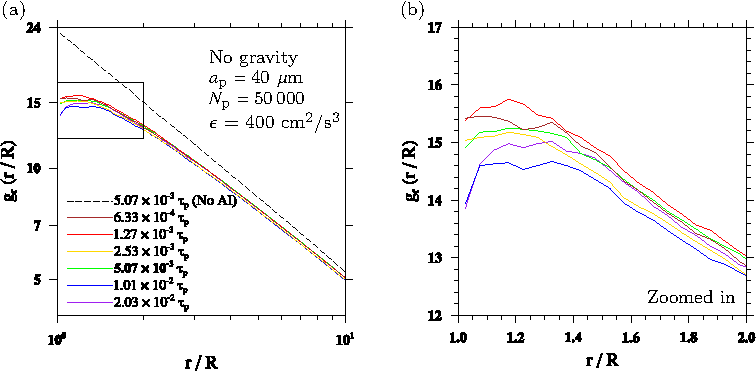
\includegraphics[width=\textwidth]{../figs/JFM/fig4.pdf}
\caption{Radial distribution function computed using different time step sizes
for the normalized separation distance in the range (a) $1 < r/R < 10$ and (b) $1 < r/R < 2$
 with the set of droplets $a_\mathrm{p} = 40~\mathrm{\mu m}$ and $N_\mathrm{p} = 50\,000$.
The black rectangle in (a) marks the region that is enlarged and shown in (b).}
\label{Fig4}
\end{figure}%------------------------------------

In the next step, we address sensitivity of the particle clustering to $\Delta t$. The RDFs computed in the same numerical simulations are shown in Figure~\ref{Fig4}. As before, Figure~\ref{Fig4}(b) presents the RDF for near-contact separation distances. Similar to the RRV, in general the RDF does not change much for different time step sizes. The only difference is observed at separation distances comparable to the particles radii. The RDF increases as the time step decreases, which is a consequence of including the lubrication forces. As already discussed, the relative velocity decreases at shorter $\Delta t$, which in turn enhances the tendency of pairs of droplets to stay together, thereby augmenting their average concentration, especially at short distances.


\begin{figure}%----------- F I G U R E ----------
\center
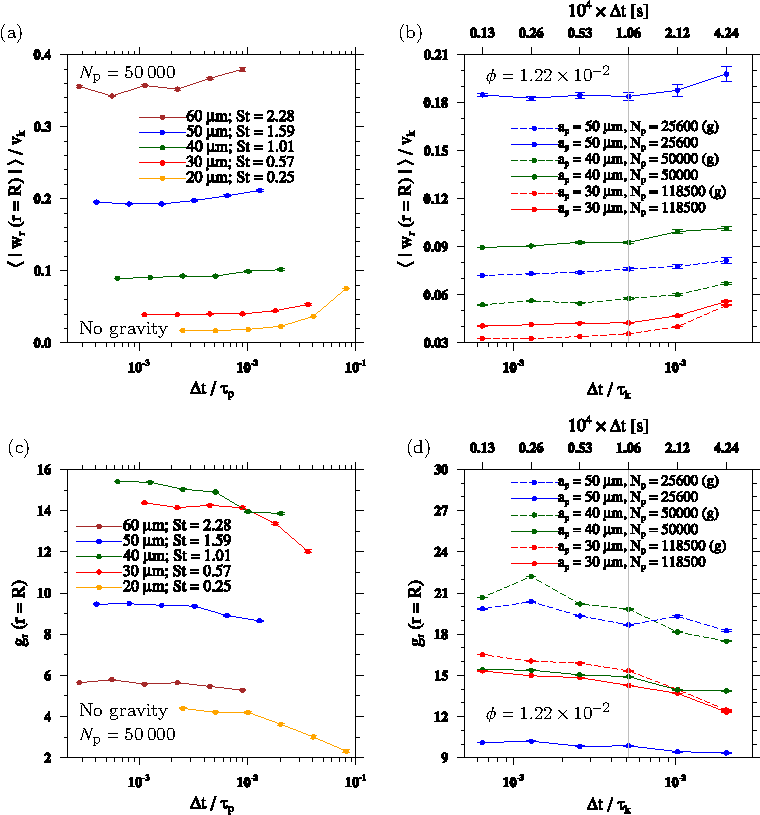
\includegraphics[width=\textwidth]{../figs/JFM/fig5.pdf}
\caption{The effect of time step size on the radial relative velocity at contact for (a) the same number of droplets: $N_\mathrm{p} = 50\,000$ and (b) the same mass loading:  $\phi = 1.22\times10^{-2}$, as well as radial distribution function at contact for (c) the same number of droplets: $N_\mathrm{p} = 50\,000$ and (d) the same mass loading: $\phi = 1.22\times10^{-2}$, considering various sets of same-size droplets with different radii, (g) stands for simulations with gravity.}
\label{Fig5}
\end{figure}%------------------------------------

The above analysis were performed for systems with a fixed liquid water content and droplets of the same radii: $a_\text{p} = 40~\mu$m. Here we extend the analysis and consider systems with particles of different radii with various or identical mass loadings. Since the lubrication forces are important mainly at short separation distances, the current analysis is restricted to the kinematic collision statistics of the droplets at contact. Figure~\ref{Fig5}(a) shows the RRV, normalized by the Kolmogorov velocity scale, of the sets of droplets with five different radii simulated with different $\Delta t$. It is important to note that the simulations in Figures~\ref{Fig5}(a) and (c) were performed with the same number of droplets, so that the mass loading in individual series is different. Even though the number of droplets is the same, the difference in the size of droplets changes the mass loading. Consequently, simulations with identical mass loading, $\phi = 1.22\times10^{-2}$, were performed as well, and the results are presented in Figures~\ref{Fig5}(b) and (d), with $\Delta t$ being normalized by $\tau_\text{K}$, directly corresponding to the set of six time steps chosen and listed on the top horizontal axes. The results shown in Figures~\ref{Fig5}(a) and (b) allow us to conclude that RRVs increase with $\Delta t$. As expected, the larger increase is observed for particles of lower inertia, which is consistent with Figure~\ref{Fig2}. It is also noteworthy to mention that the sensitivity of these statistics to $\Delta t$ depends on both the droplet inertia and gravity. The increase in RRV is not strictly related to the aerodynamic interactions, since in both series of simulations the same mass loading was considered. The enhancement of RRV at larger $\Delta t$ should be understood as a more effective decorrelation of droplet motion caused by a coarser sampling of the background fluid velocity. In simulations without gravity the RRV is dominated by so-called path-history or non-local effects. Gravity alters this mechanism and reduces the correlation between fluid and particles. This is most likely the reason why for droplets of radii 30--40~$\mu$m a slightly larger sensitivity is observed in simulations with gravity. For heavier droplets, i.e.\ 50~$\mu$m the dependency of the kinematic statistics, especially the RRV, to $\Delta t$ is larger if gravity is not considered. This is because gravity reduces the droplets' velocity fluctuations (relative to the fluid). Thus, the RRV is less dependent on $\Delta t$. In the limiting case of particles with infinite inertia, the turbulence effects on the RRV are negligible, and the constraints on the time step become insignificant.

Corresponding to Figures~\ref{Fig5}(a) and (b), RDFs of systems with the same number of droplets and the same mass loading are shown in Figures~\ref{Fig5}(c) and (d), respectively. An opposite decreasing trend is observed for the at-contact RDFs. Again, the observed dependencies can be interpreted as consequences of including the lubrication forces. Large time steps do not allow adequate capturing of the short-range aerodynamic forces, so that the effect of particle hampering is smaller and consequently the RRV is overestimated. Larger RRV results in higher probability of particle collision. This in turn has an indirect effect on reducing the RDF, since after every collision one of the droplets is moved to a new location so that, in an average sense, the droplets have a more uniform distribution, leading to smaller RDFs. 

\begin{figure}%----------- F I G U R E ----------
\center
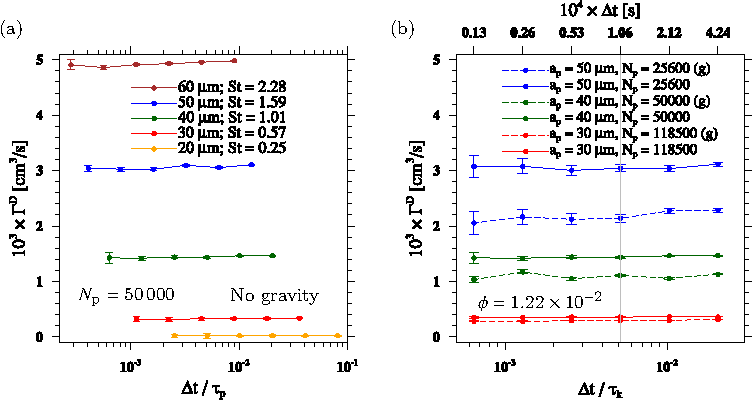
\includegraphics[width=\textwidth]{../figs/JFM/fig6.pdf}
\caption{The effect of time step size on the dynamic collision kernel for (a) the same number of droplets: $N_\mathrm{p} = 50\,000$ and (b) the same mass loading: $\phi = 1.22\times10^{-2}$, considering various sets of same-size droplets with different radii.}
\label{Fig6}
\end{figure}%------------------------------------

Since the effect of the time step size is different for the RRV and RDF, the question arises about the net effect of $\Delta t$ on the collision kernel---the parameter directly proportional to the collision rate. The values of the dynamic collision kernel with respect to different time step sizes are presented in Figure~\ref{Fig6}. Contrary to the kinematic statistics, the dynamic collision kernel does not show considerable changes with the time step size. This may be explained as a result of the mutual compensation of these two opposite effects. Here, it is worth referring to the kinematic definition of the collision kernel, namely $\Gamma^\text{K}$ (Equation \ref{eq:38}), which is proportional to the product of the RRV and RDF. This experiment shows that even though the dynamical characteristics are similar for different choices of $\Delta t$, the kinematic statistics may be different. In Figure~\ref{Fig6}(b) we observe an increase in numerical uncertainty with the droplet radii. This larger uncertainty especially in the collision kernels of 50~$\mu$m droplets is due to fewer number of detected collisions, which itself is a direct result of lower number of drops used in these simulations to maintain the same mass loading.

The above considerations lead to the final conclusion that for time steps smaller than $\Delta t=1.06\times10^{-4}$~s, the changes in the kinematic and dynamic statistics are rather insignificant. Thus, the rest of simulations in this subsection are conducted with this time step size.



\subsubsection{Matching point between short- and long-range interaction}
As already pointed out, standard HDNS is not capable of accurately representing the AI forces acting on spherical particles if the separation distance between them is smaller than or comparable to their mean radius (see Figure~\ref{Fig1}). To overcome this problem, a new numerical model has been proposed in which computation of the drag forces switches from HDNS to the exact formulation of \citet{JO84} at a heuristically chosen matching point. To maximize fidelity of our model, the location of the matching point for these two approaches should be properly optimized.

It should be recalled that the exact formulation of \citet{JO84} has been derived for two rigid spheres immersed in a viscous fluid and is limited to the Stokes regime. Therefore, this approach is suitable for modeling a binary system of interacting particles. Still, this binary treatment can be accurate for simulating multiphase flows if the volume fraction of the dispersed phase is relatively small. In such systems there is a low probability of three or more droplets simultaneously being at a separation distance comparable to their radii. On the other hand, this exact treatment is binary and thus unable to capture the effects of many-body interactions among particles, while these effects can be faithfully handled under HDNS approach. Considering the upsides and downsides of these two approaches, an optimal location for the matching point of them needs to be found.

\begin{figure}%----------- F I G U R E ----------
\center
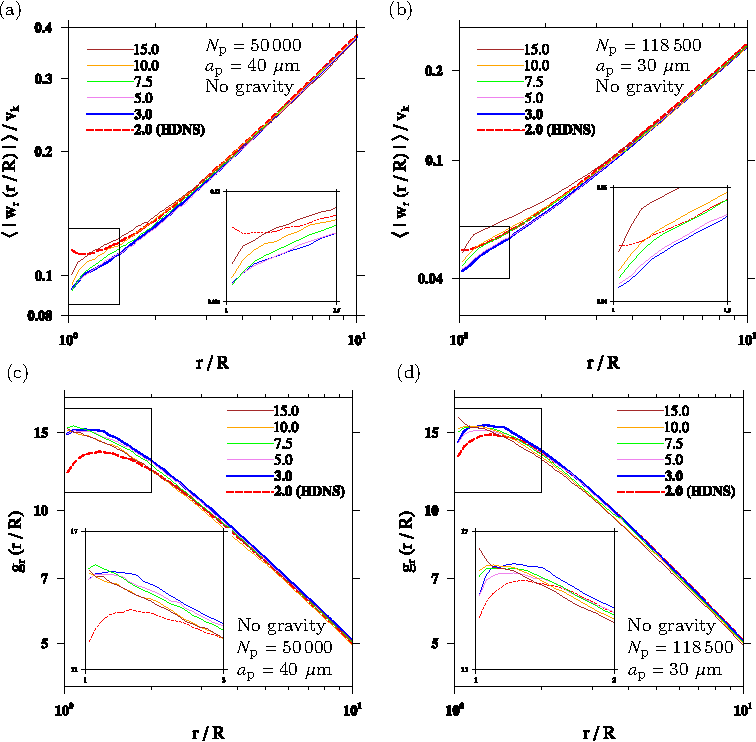
\includegraphics[width=\textwidth]{../figs/JFM/fig7.pdf}
\caption{Variations in the radial relative velocity (a,b) as well as radial distribution function (c,d) for the sets of droplets (a,c) $a_\mathrm{p} = 40~\mathrm{\mu m}, N_\mathrm{p} = 50\,000$, and (b,d) $a_\mathrm{p} = 30~\mathrm{\mu m}, N_\mathrm{p} = 118\,500$ when the lubrication forces are considered within different ranges of interaction $\delta$.}
\label{Fig7}
\end{figure}%------------------------------------

The optimization procedure consists of comparing collision statistics, both kinematic and dynamic, from a series of simulations performed with different choices of $\delta$. First, we analyze the RRV and RDF at different separation ranges, namely, $1<r/R<10$. This is a necessary step, since the choice of $\delta$ may have some impact on the statistics. Figure~\ref{Fig7} shows the normalized RRV and RDF of two monodisperse systems containing droplets of different radii/inertia but the same mass loading: $\phi = 1.22\times10^{-2}$. The range of considered $\delta$ extends from 2 to 15. In Figure~\ref{Fig7}(a) and (b) a noticeable reduction in the RRV is seen as soon as the binary formulation is applied within separation distances $s<\delta=3$. This is more obvious in the near-contact region which is marked and enlarged for each Figure. A slight but systematic growth in the relative velocity is observed in simulations with larger $\delta$. Surprisingly, for a larger $\delta$, or equivalently a larger range of exact binary treatment, the RRV approaches the solution computed with the standard HDNS. This result may be counterintuitive and has to be interpreted along with the RDF. The corresponding values of the RDF increase with $\delta$, which can be explained as an effect of stronger droplet hampering due to the lubrication effect. This in turn results in a more intense clustering at droplet size scales. Stronger clustering and shorter separation distances enhance the effect of relative motion due to many-body interactions. It is important to note that $g_r(r=R)$ computed using the coupled model when $\delta = 3$ is significantly larger than the corresponding value from the standard HDNS, i.e.\ $\delta = 2$. The results suggest that it is justified to use the exact binary treatment for $s<3$.

\begin{figure}%----------- F I G U R E ----------
\center
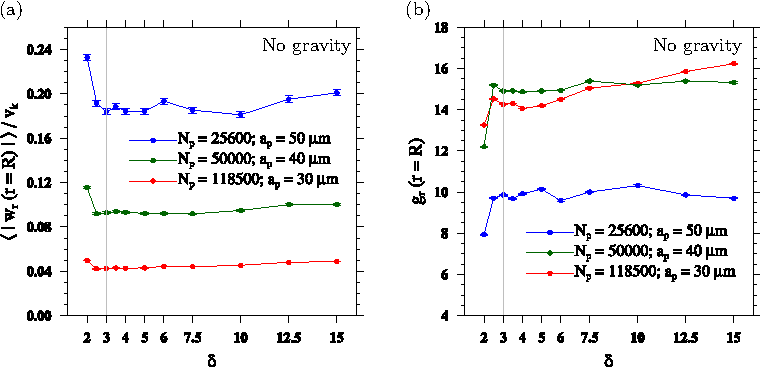
\includegraphics[width=\textwidth]{../figs/JFM/fig8.pdf}
\caption{Variations in the (a) at-contact radial relative velocity and (b) at-contact radial distribution function for three sets of droplets with the same mass loading, $\phi = 1.22\times10^{-2}$, when the lubrication forces are considered within different ranges of interaction.}
\label{Fig8}
\end{figure}%------------------------------------

In Figure~\ref{Fig8}, we present at-contact RRV and RDF computed for three systems with different droplet radii but the same mass loading. Again, the binary treatment is applied within different ranges of separation distances such that $\delta=2$ indicates the standard HDNS approach. RRVs at contact show a decline when the lubrication forces are included for separation distances smaller than $\delta=3$. This confirms that the lubrication interaction prevents the particles from both approaching and receding from each other. The decrease in $\langle |w_r(r=R)| \rangle$ depends on the droplet inertia, being more noticeable for the larger droplets. This effect can be attributed to a stronger decorrelation of the fluid and particle velocities. Looking at Figure~\ref{Fig8}(b), at-contact RDFs indicate stronger clustering when the lubrication forces are considered because the reduction in RRV allows the droplets to stay longer at closer separations.

\begin{figure}%----------- F I G U R E ----------
\center
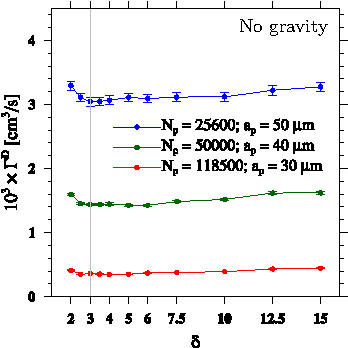
\includegraphics[width=0.6\textwidth]{../figs/JFM/fig9.pdf}
\caption{Variations in the dynamic collision kernel for three sets of droplets with the same mass loading, $\phi = 1.22\times10^{-2}$, when the lubrication forces are considered within different ranges of interaction.}
\label{Fig9}
\end{figure}%------------------------------------

For completeness of the analysis, we present the dynamic collision kernels of these three systems modeled with different $\delta$ in Figure~\ref{Fig9}. As expected, the dynamic collision kernel is reduced when the lubrication forces are considered. In other words, ignoring the effect of lubrication leads to an overestimation of the collision rate. This reduction is mainly due to smaller values of the radial relative velocities between droplets. It is interesting to note that for $\delta=3$ the relative reduction in $\Gamma^\text{D}$ is smaller than that in the RRV. This mitigation is mainly due to stronger clustering, demonstrated by the larger values of the RDF at contact presented in Figure~\ref{Fig8}(b).



\subsubsection{Kinematic and dynamic collision statistics}
Here, the effect of lubrication interaction on the droplet collision statistics is discussed more broadly. Particularly, we analyze the role of lubrication forces in systems with droplets of different inertia. The range of droplet radii considered in these simulations varies from 20 to 60~$\mu$m. Moreover, the simulations have been performed for a wide range of energy dissipation rates: 10--400~cm$^2$/s$^3$. The results from the new implementation of HDNS with lubrication forces are compared with the simulations from the standard HDNS, those without aerodynamic interactions, and the results from other studies as well as theoretical estimations.

\begin{figure}%----------- F I G U R E ----------
\center
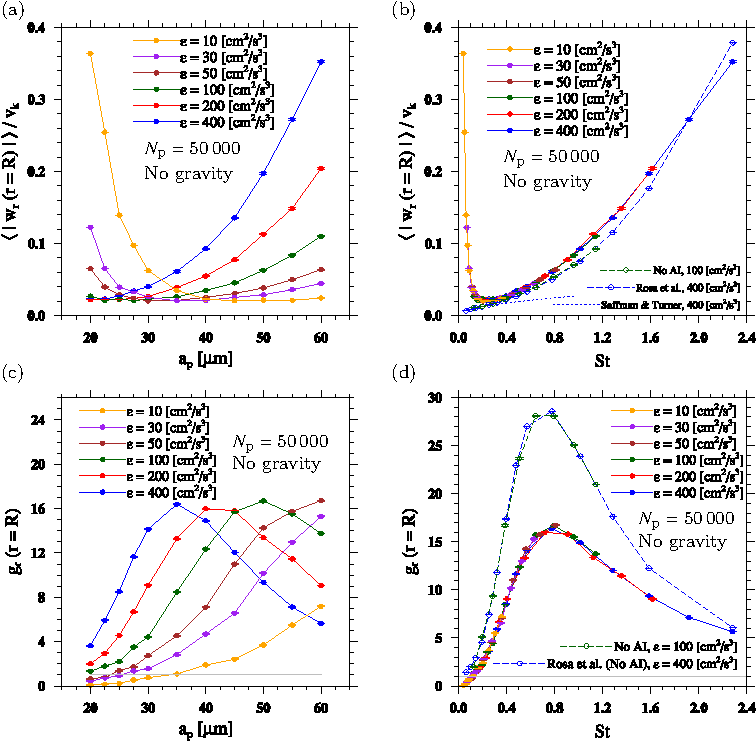
\includegraphics[width=\textwidth]{../figs/JFM/fig10.pdf}
\caption{The effect of turbulent energy dissipation rate on the at-contact radial relative velocity for different (a) droplet sizes and (b) Stokes numbers, and its effect on the at-contact radial distribution function for different (c) droplet sizes and (d) Stokes numbers. In (b) the theoretical model of \cite{ST56} is shown. The DNS results of \cite{RPAGW13}: Figures~8(a) \& 13(a), are additionally included in (b) and (d).}
\label{Fig10}
\end{figure}%------------------------------------

First, we address the effect of the energy dissipation rate on the kinematic and dynamic collision statistics in the absence of gravity. Figure~\ref{Fig10} shows the at-contact RDFs and RRVs of monodisperse systems computed in six series of simulations each at a different $\epsilon$. In all these simulations the number of droplets was fixed and equal to $N_\text{p} = 50\,000$. Additionally, the results are plotted against the Stokes number, which is a function of both the size of the droplet and turbulent energy dissipation rate. The Stokes number is a quantitative measure of the droplet inertia. With such scaling all the lines collapse to one U-shaped line with a minimum roughly at $St = 0.2$. The three additional curves shown there correspond to: (i) the current implementation for the same set of droplets at $\epsilon = 100~\mathrm{cm^2/s^3}$ but without aerodynamic interactions, (ii) the data from the study of \cite{RPAGW13}: Figure~13(a), and values from the theoretical model by \cite{ST56} valid in the limiting case of zero-inertia particles. The results in Figure~\ref{Fig10}(a) show that the RRVs are highly sensitive to $\epsilon$ in the limit of both very small and large droplets, but in a different manner. As for the large droplets, e.g.\ 60~$\mathrm{\mu m}$, this increase can be explained as the effect of larger inertia. The motion of such droplets is weakly correlated with the background flow, and consequently the RRV is larger. 

More interestingly, an opposite trend is observed for the smaller droplets. The average RRV at contact increases when the energy dissipation rate decreases. In Figure~\ref{Fig10}(b), for $St < 0.2$ there is a sharp increase in the RRVs since only pairs of droplets with considerably large relative velocities are able to break through the barrier of lubrication forces. This, however, does not happen frequently, as can be deduced from Figure~\ref{Fig10}(d). The values of the RDF at contact for $St < 0.2$ are very low, which means that only a small number of droplets can become nearly touching. Figure~\ref{Fig10}(c) shows that the values of at-contact RDFs computed using different $\epsilon$ follow a bell-shaped line. As the energy dissipation rate decreases, the bell stretches and the maximum shifts towards the larger droplets. In Figure~\ref{Fig10}(d) the RDFs are plotted also as a function of the Stokes number, exhibiting a maximum approximately at $St = 0.8$. 

The key finding, here, concerns differences between the standard simulations under one-way momentum coupling and those with full representation of aerodynamic forces. As for the RRV we observe a certain similarity of both models in the range $St>0.2$. A minor increase in RRV for droplets with $St<1.9$ can be seen, as well as a little reduction for droplets of larger inertia if the interaction forces are considered. For $St<0.2$ the differences between different approaches are large, but statistically insignificant, due to rarity of situations when two particles are close to each other. The lubrication forces as well as the long range many-body interactions have significant effects on the RDF. For droplets of $St=0.8$ the difference in the RDF reaches almost 50\%. There are two reasons for this reduction. First, the lubrication forces prevent the particles from approaching each other. Second, in the simulations with aerodynamic interactions after each collision one of the droplets is relocated, decreasing local droplet number density, whereas in simulations under one-way momentum coupling droplets are allowed to overlap.

\begin{figure}%----------- F I G U R E ----------
\center
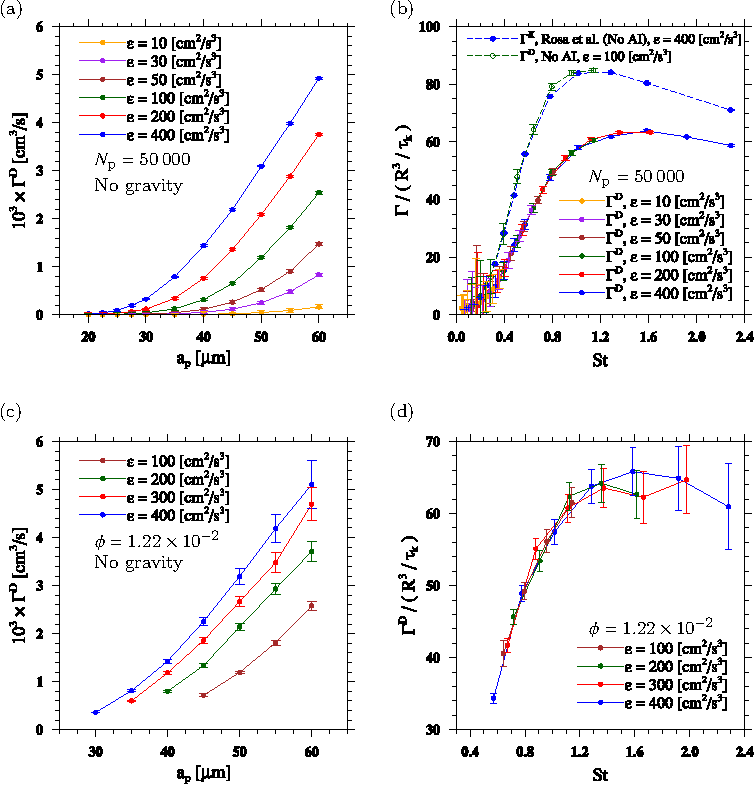
\includegraphics[width=\textwidth]{../figs/JFM/fig11.pdf}
\caption{The dynamic collision kernel as function of droplet size in flows with different energy dissipation rates for (a) $N_\mathrm{p} = 50\,000$ and (c) $\phi = 1.22\times10^{-2}$, and the normalized dynamic collision kernel for corresponding values of the Stokes number, also for (b) $N_\mathrm{p} = 50\,000$ and (d) $\phi = 1.22\times10^{-2}$. The results of \cite{RPAGW13} are added to panel (b) for comparison.}
\label{Fig11}
\end{figure}%------------------------------------

In addition to the two-point collision statistics, the dynamic collision kernel, $\Gamma^\text{D}$, is computed for the same sets of simulations and presented in Figure~\ref{Fig11}. According to the data in Figures~\ref{Fig11}(a) and (c), the collision kernel increases monotonically both with the droplet radius and the energy dissipation rate. Since both parameters correspond to larger Stokes numbers, or equivalently larger inertia, the droplets collide more frequently due to higher relative velocities. The normalized values of the dynamic collision kernel are presented in Figures~\ref{Fig11}(b) and (d) as a function of the Stokes number. Within a numerical uncertainty, all values collapse to a single curve showing an increase with the Stokes number until $St = 1.6$. For larger $St$, a slight reduction is noticeable. The increasing trend is largely due to the augmentation of relative velocities with the Stokes number (see Figure~\ref{Fig10}(b)) while the decreasing trend stems from the reduction in the clustering of droplets (see Figure~\ref{Fig10}(d)).

Finally, we address the differences between simulations with and without aerodynamic interactions. Figure~\ref{Fig11}(b) shows a comparison of $\Gamma^\text{D}$ computed using the new model with results obtained from simulations under one-way momentum coupling. Based on the data, it can be claimed that the collision kernel and consequently the collision rate of monodisperse systems are smaller if the aerodynamic interactions are considered. The reduction is generally a function of the particle inertia. Specifically, for droplets of $St=1$ the reduction is about 25\%. The above results together suggest that this effect should be parameterized in future NWP models. 

\subsubsection{HDNS with lubrication vs.\ HDNS vs.\ DNS}
This part the discussion gives a closer insight into the differences between three numerical approaches. We compare collision statistics computed using (i) the new model with full representation of the short-range interreacting forces, (ii) standard HDNS approach and (iii) simulations under one-way coupling in which the effect of aerodynamic interactions is neglected.

\begin{figure}%----------- F I G U R E ----------
\center
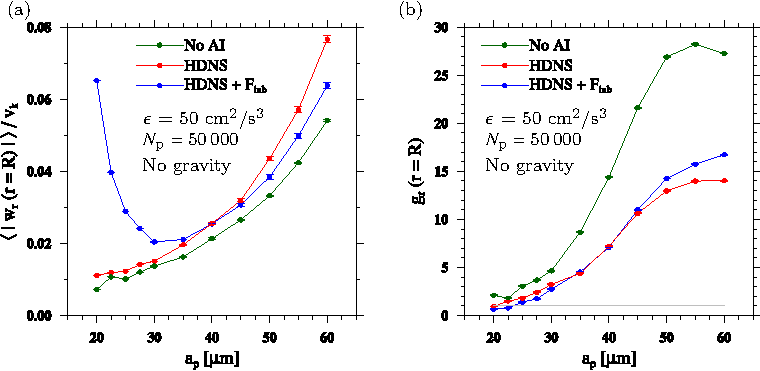
\includegraphics[width=\textwidth]{../figs/JFM/fig12.pdf}
\caption{Changes in the at-contact (a) radial relative velocities and (b) radial distribution functions when the effect of lubrication forces is taken into consideration compared with the standard HDNS without lubrication effects as well as the case without aerodynamic interaction for $N_\mathrm{p} = 50\,000$ droplets in a flow at a low dissipation rate $\epsilon$ = 50~cm$^2$/s$^3$.}
\label{Fig12}
\end{figure}%------------------------------------

Figure~\ref{Fig12} shows (a) the normalized RRVs and (b) RDFs at contact as a function of the droplet radius. The three series of simulations were performed using different numerical approaches and the same settings. Both the number of droplets ($N_\mathrm{p} = 50\,000$) and the energy dissipation rate ($\epsilon$ = 50 cm$^2$/s$^3$) were fixed in all simulations. The gravitational settling of the droplets was not considered.

The obtained results are consistent with previous observations. The RRV is significantly augmented in the range of smaller droplets if the lubricative forces are included. Although the effect of lubrication is clearly visible in the RRV, in an average sense, this sharp increase does not have much influence on the collision statistics (see Figure~\ref{Fig11}) since the number of detected pairs at short separation distances is very small. This can be confirmed by looking at Figure~\ref{Fig12}(b) showing  RDFs at contact for the same range of sizes. For larger droplets the RRV computed with the new approach falls in between two other models. The increase over the simulations without aerodynamic interactions is a combined effect of short-range lubrication forces and many-body interactions. The most pronounced enhancement of the RRV was obtained in hybrid DNS. This result is rather expected since in HDNS the motion of the particles is not hampered by the lubricating forces.

Figure~\ref{Fig12}(b) shows a considerable reduction in at-contact RDFs when aerodynamic interactions among droplets are considered. However, in other studies, e.g.\ \cite{BKL97} and \cite{YKHC18}, an opposite trend was reported indicating that aerodynamic interactions enhance RDF. We believe that this discrepancy is due to some numerical effects resulting from assumptions made here. An influential part of the code used in the present study is the droplet relocation module. The module determines a new random location for one of the droplets of colliding pair. This treatment mimics the well-known physical process, in which two colliding droplets form a larger drop. This large drop does not belong to the considered size class. At the same time a new droplet formed by diffusion or collision--coalescence is introduced into the domain. By turning this module on, even if the aerodynamic interactions are not considered, the mechanism of clustering is ``artificially'' altered, and the droplet distribution tends to become more uniform. Consequently, the RDF values are smaller. It should also be emphasized that for the largest droplets $(60~\mathrm{\mu m})$ the RDF at contact is slightly larger if lubrication is added. This demonstrates that the lubrication interaction of such droplets prevents their collisions more efficiently.

\begin{figure}%----------- F I G U R E ----------
\center
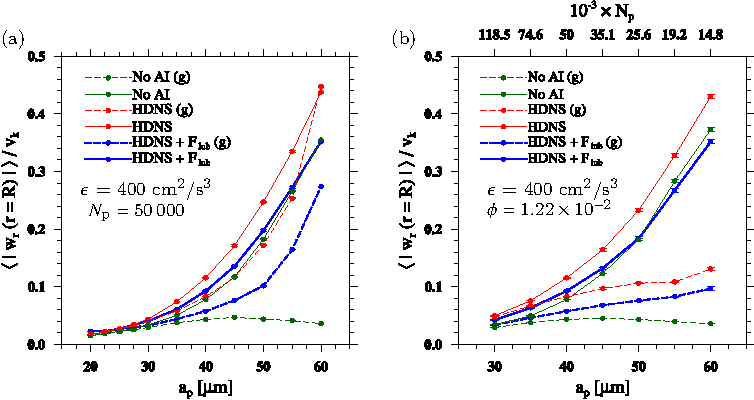
\includegraphics[width=\textwidth]{../figs/JFM/fig13.pdf}
\caption{Comparison of at-contact radial relative velocity in case when there is aerodynamic interaction, both including and excluding lubrication forces, and when there is no aerodynamic interaction, all with and without gravity, for (a) the same number of droplets: $N_\mathrm{p} = 50\,000$ and (b) the same mass loading: $\phi = 1.22\times10^{-2}$ at the dissipation rate $\epsilon$ = 400 cm$^2$/s$^3$.}
\label{Fig13}
\end{figure}%------------------------------------

Figure~\ref{Fig13} compares the RRV of monodisperse systems at a higher energy dissipation rate equal to $\epsilon = 400~\mathrm{cm^2/s^3}$. Again, the simulations were performed using different numerical approaches but this time we separately considered the cases with and without gravity. Since the effect of the droplet mass loading may be important the analysis includes both the simulations at a fixed number of droplets, Figure~\ref{Fig13}(a), and at a fixed mass loading, Figure~\ref{Fig13}(b). Obtained results show that, compared to the standard HDNS, the RRV decreases when the additional effect of lubrication is taken into consideration. This is due to the larger drag forces that are inherently not accounted for by the HDNS. Moreover, there is a general increase in the relative velocity with the size of droplets, which arises from the higher inertia of larger droplets that enables them to move more independently from the background flow field. There is, however, an exception in the case without aerodynamic interactions and with gravity, which shows a reduction of RRV for droplets larger than $45~\mathrm{\mu m}$. This phenomenon was reported in several former studies \citep[see][]{RPAGW13, RPAW15, IBC16}. Its physics is non-trivial, since for monodisperse systems, there is no differential sedimentation and the effect of gravity on the particle-pair motion is entirely implicit. In contrast to bidisperse systems \citep{DB18}, the effect of particle settling does not offset the effect of turbulent mixing. \cite{IBC16} presented physical arguments explaining this mechanism, namely, gravity suppresses the non-local contribution to the particle relative velocities by reducing the correlation timescale of the flow experienced by the particles. Therefore, the average relative velocity of the droplets is lower than in simulations without gravity. The effect of gravity on the RRV is negligible for droplets smaller than $30~\mathrm{\mu m}$. Moreover, for such small droplets, at $\phi = 1.22\times10^{-2}$ or lower, the effect of aerodynamic interaction may be practically neglected. This is likely due to stronger correlation of such particles with the turbulent flow. The motion of low inertia particles is dominated by the turbulent flow and the aerodynamic interactions among them do not have a considerable impact.

\begin{figure}%----------- F I G U R E ----------
\center
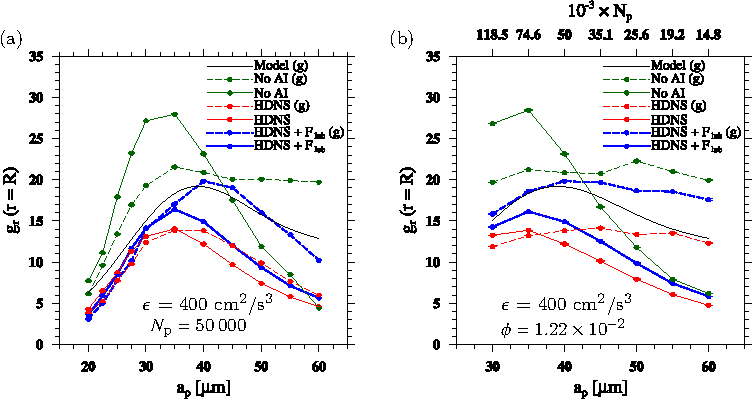
\includegraphics[width=\textwidth]{../figs/JFM/fig14.pdf}
\caption{Comparison of at-contact radial distribution function when there is aerodynamic interaction, both including and excluding lubrication forces, and when there is no aerodynamic interaction, all with and without gravity, for (a) the same number of droplets: $N_\mathrm{p} = 50\,000$ and (b) the same mass loading: $\phi = 1.22\times10^{-2}$ at the dissipation rate $\epsilon$ = 400 cm$^2$/s$^3$. The empirical model of \cite{ARW08}: Equations 84 \& 85 for $R_{\lambda}=76.86$, is also included for comparison.}
\label{Fig14}
\end{figure}%------------------------------------

Including aerodynamic interactions into the model has a direct impact on the kinematic collision statistics making the RRV more closely dependent on the RDF and vice versa. This can be explained with an example, namely, an enhanced RRV increases collision rate and consequently enforces redistribution of particles. In simulations without aerodynamic interactions particles can overlap, so this redistribution is not needed. To quantify this phenomenon the changes in RRVs have to be examined together with changes in RDFs. Figure~\ref{Fig14} shows the RDF complementary to the RRV (plotted in Figure~\ref{Fig13}) calculated in the same series of simulation. As expected, the largest values of the RDF were obtained in simulations without aerodynamic interactions. In turn, in simulations with aerodynamic interactions the RDFs depend on the mass loading. For systems at a fixed number of droplets (see Figure~\ref{Fig14}(a)) the differences between simulations with lubrication forces and standard HDNS appear for droplets larger than $30~\mathrm{\mu m}$. According to these results there is stronger clustering at short length scales when the effect of lubrication is taken into account, especially together with gravity. In simulations at fixed mass loadings the offset in the RDF is almost constant for all considered droplet radii.

\begin{figure}%----------- F I G U R E ----------
\center
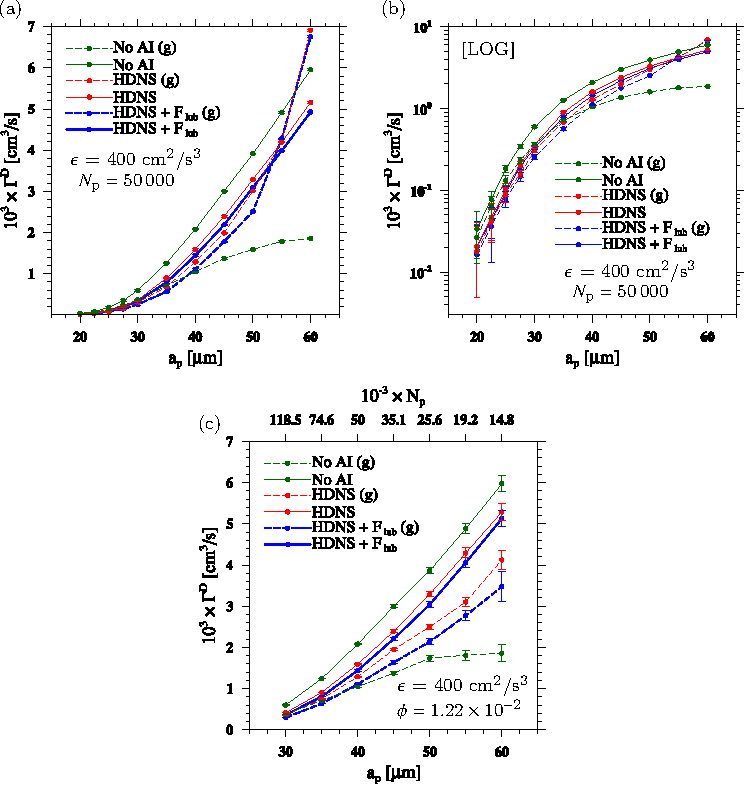
\includegraphics[width=\textwidth]{../figs/JFM/fig15.pdf}
\caption{Comparison of the dynamic collision kernel when there is aerodynamic interaction, both including and excluding lubrication forces, and when there is no aerodynamic interaction, all with and without gravity, for (a) the same number of droplets: $N_\mathrm{p} = 50\,000$ in linear scale and in (b) logarithmic scale, and for (c) the same mass loading: $\phi = 1.22\times10^{-2}$ at the dissipation rate $\epsilon$ = 400~cm$^2$/s$^3$.}
\label{Fig15}
\end{figure}%------------------------------------

Figure~\ref{Fig15} presents the dynamic collision kernels of the cases considered above for $\epsilon = 400~$cm$^2$/s$^3$. In general, the collision kernel is a monotonic and increasing function of the droplet radii. This increase of $\Gamma^\text{D}$ is mainly due to larger values of RRVs which is a consequence of larger particle inertia. The lubrication forces slightly reduce the collision kernel, which again stems from the reduction in the relative velocities. The RRVs are smaller when the lubrication force between pairs is taken into account. For each size of droplets, the lowest collision kernel is usually for sedimenting droplets and the highest for non-sedimenting droplets if there is no aerodynamic interaction. When the aerodynamic interaction is considered, the collision kernels lie in between, being slightly lower for the sedimenting droplets. This is not general, however, since the mass loading is important, too. Accordingly, the results for the mass loading $\phi = 1.22\times10^{-2}$ are shown in Figure~\ref{Fig15}(c). The effect of mass loading on the collision statistics of droplets will be discussed in more detail.



\subsubsection{Validation of corrected kinematic formulations}

\begin{figure}%----------- F I G U R E ----------
\center
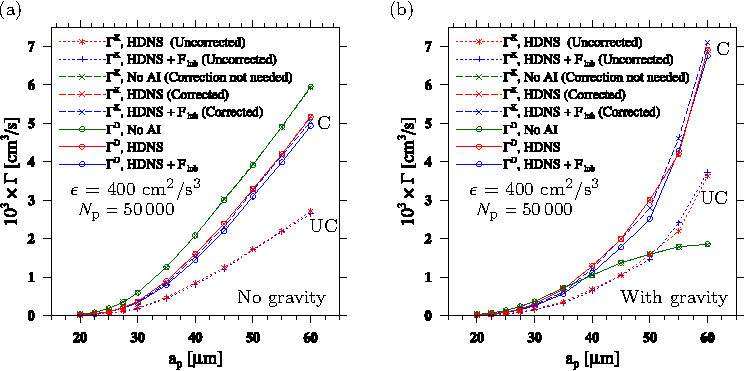
\includegraphics[width=\textwidth]{../figs/JFM/fig16.pdf}
\caption{Comparisons between the collision kernel obtained from the dynamic formulation with that computed using the kinematic formulation, both before (UC) and after (C) applying corrections, when (a) gravity is not considered and (b) when there is gravity.}
\label{Fig16}
\end{figure}%------------------------------------

The RRVs and RDFs presented in this study are subjected to the corrections given in Equations~(\ref{eq:34})--(\ref{eq:37}) provided by \cite{WAKG05}. In Figure~\ref{Fig16}, the collision kernels computed using the corrected kinematic statistics at contact, Equation~(\ref{eq:38}), are benchmarked against the dynamic collision kernels, Equation~(\ref{eq:33}) computed in the simulations with and without gravity. In simulations without aerodynamic interactions, the correction is not needed because particles can overlap, hence the volumetric rate of collisions is equal to the influx of particles from the surface area of the collision sphere. Consequently, $\Gamma^\text{D}$ and $\Gamma^\text{K}$ in Figure~\ref{Fig16} perfectly overlap.

However, for the cases where there is aerodynamic interaction, the relocation mechanism changes the influx through the collision sphere by creating a particle-free zone behind it. In such a case, standard kinematic formulation leads to an inconsistency with the dynamic formulations. In Figure~\ref{Fig16} the kinematic collision kernels are presented both before (UC - uncorrected) and after (C - corrected) applying the corrections. We find that after correction the kinematic and dynamic collision kernels are in a quantitative agreement. It should be noted, however, that there is a small but visible difference between $\Gamma^\text{K}$ and $\Gamma^\text{D}$ in simulations performed with full representation of the lubrication forces. We hypothesize that this discrepancy may have two sources. First, numerical methods have some intrinsic limitations, so that the values of RDF and RRV at contact can be evaluated with a finite accuracy. In this particular case, the RDF may be somewhat overestimated. Second, the average statistics of these simulations were calculated using fewer samples. As shown in Figure~\ref{Fig15}, $\Gamma^\text{D}$ is consistently smaller in simulations with lubrication forces comparing to standard HDNS. This means that particles collide less frequently, which in turn might result in larger numerical uncertainty in these statistics. Overall, the investigation shows that these geometric corrections must be included in simulations when the particles are displaced after collisions.



\subsubsection{Effect of particles number density and mass loading}

\begin{figure}%----------- F I G U R E ----------
\center
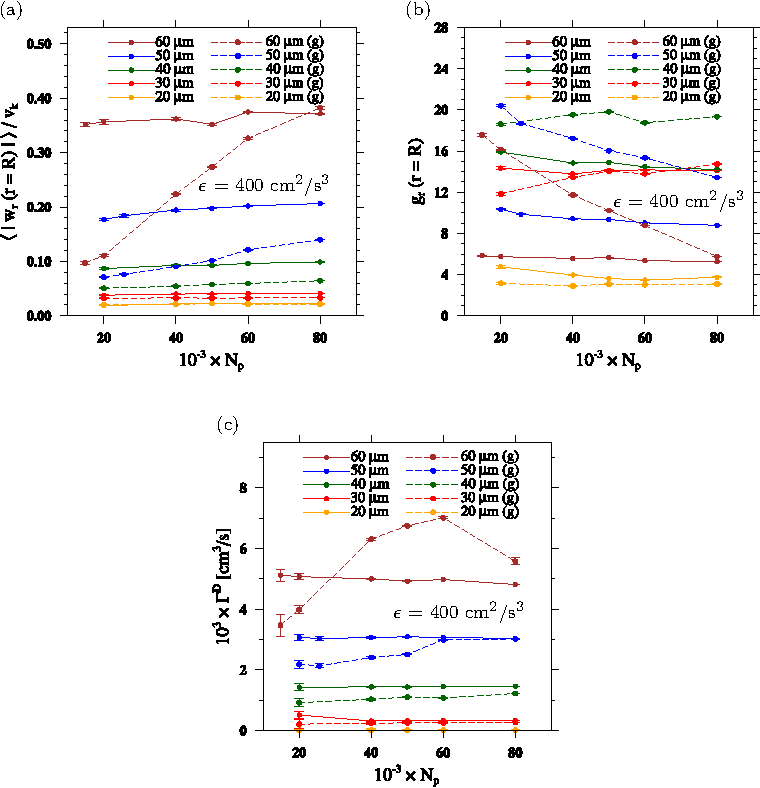
\includegraphics[width=\textwidth]{../figs/JFM/fig17.pdf}
\caption{Changes in the at-contact (a) radial relative velocity, (b) at-contact radial distribution function, and (c) the dynamic collision kernel for the sets of droplets with different radii and numbers, i.e.\ different mass loadings.}
\label{Fig17}
\end{figure}%------------------------------------

Finally, we examine the effect of droplet mass loading on the kinematic and dynamic collision statistics. Figure~\ref{Fig17} shows at-contact RRVs and RDFs together with corresponding values of the dynamic collision kernels computed in simulations with different number of droplets. The considered systems were monodisperse and contained droplets of radii between 20--60~$\mathrm{\mu m}$. 

The results presented in Figure~\ref{Fig17}(a) confirm observations reported in former studies \citep[e.g.][]{RPAGW13} that inertia enhances the RRV between closely separated particles. It stems from the fact that particles of larger inertia retain their kinetic energy longer than corresponding fluid elements, therefore their relative motion is more strongly decorrelated. Gravity noticeably reduces the velocity correlation between fluid and particles and thus diminishes the non-local effects \citep{IBC16}. Consequently, the RRV of larger droplets is significantly lower. In simulations with $N_\mathrm{p} = 20\,000$ of 60~$\mathrm{\mu m}$ droplets, gravity reduces the radial relative velocity by about 3 times. This is the regime in which the effect of the aerodynamic interaction is relatively weak. In simulations with larger number of droplets, or equivalently larger mass loadings, the aerodynamic interactions gain importance and alter dynamics of the entire systems. As the mean distance between the droplets decreases the additional forces result in a stronger decorrelation of the particle motion but mainly in simulations with gravity. Therefore, we observe a monotonic increase in RRV with the particle number density. The slopes of these dashed lines decrease with the size of the droplets, which is a consequence of smaller mass loadings. (The simulations were performed at fixed $N_\mathrm{p}$.) Thus, the effect of aerodynamic interactions is weaker. Interestingly, this effect is much smaller in simulations without gravity. This is rather expected since the RRV in simulations without gravity is already very large such that the aerodynamic interaction does not result in further enhancement of the particle relative motion.

An opposite, i.e.\ decreasing, trend is observed for the RDFs visualized in Figure~\ref{Fig17}(b). For most simulated cases the RDF decreases with $N_\mathrm{p}$. The only exceptions are systems of the middle-sized 30 and 40~$\mathrm{\mu m}$ droplets. However, the little differences fall in the range of statistical uncertainty. The decreasing trend is more pronounced for larger settling droplets. This is attributed to the enhanced relative velocities, which prevents droplet clustering, at least at particle-scale distances.

The two opposite trends present in the kinematic statistics should be also reflected in the collision kernels. Figure~\ref{Fig17}(c) shows $\Gamma^\text{D}$ as a function of the droplet number density. It indicates that the relative changes in the collision kernel for increasing $N_\mathrm{p}$ are smaller compared to the changes in the kinematic statistics. This likely results from the fact that $\Gamma^\text{D}$ is proportional to the product of the RRV and RDF. As expected, the largest sensitivity to $N_\mathrm{p}$ is observed for the largest settling droplets. Interestingly, $\Gamma^\text{D}$ of 60~$\mathrm{\mu m}$ droplets is not monotonic. For low droplet concentrations, i.e.\ up to $N_\mathrm{p} = 60\,000$, there is a systematic increase in the collision kernel, which is the effect of enhancement in RRVs. Then, for $N_\mathrm{p} > 60\,000$ the dynamic collision kernel decreases, and this corresponds to the same decreasing trend in the RDF.

\subsubsection{Summary}

The collision--coalescence of water droplets has been quantified using the combined Eulerian--Lagrangian numerical approach incorporating the exact representation of aerodynamic interactions between droplets. The numerical method combines standard HDNS approach with the exact analytical formula for the lubrication forces. Merging these two approaches allows us to jointly represent two important effects, usually neglected in studies. The HDNS accurately captures the effect of many-body interactions among widely separated droplets. In turn, the analytical solution for two interacting rigid spheres in low-Reynolds-number flows allows us to represent the lubrication effects. Impact of gravity was also considered, and the simulations have been performed for both sedimenting droplets and droplets without sedimentation. For modeling background turbulent flows, we used a computational mesh of relatively low resolution, i.e.\ $64^3$ (low Reynolds number). A reasonable numerical cost of such simulations enables obtaining particle statistics for a wide range of parameters. The main focus of this part of discussion was to analyze the effects of aerodynamic interactions on the kinematic and dynamic collision statistics rather than sensitivity to $R_{\lambda}$.

Several important conclusions can be drawn based on the results from numerical experiments. First, in the absence of gravity the aerodynamic interactions reduce the RDF, and the reduction depends on the particle inertia (see Figures~\ref{Fig4}, \ref{Fig10}(d), and \ref{Fig12}(b)). For example, for droplets with $St=0.8$ the RDF is about 50\% smaller than in analogous simulations without aerodynamic interactions. Second, the RRV is slightly enhanced, particularly in those systems with droplets of low inertia (see Figures~\ref{Fig3}, \ref{Fig10}(b), and \ref{Fig12}(a)). Consequently, the reduction in the collision kernels of interacting droplets is also a function of the Stokes number (see Figure~\ref{Fig11}(b)). Specifically, for droplets of $St$ = 1 the reduction is about 25\%. Third, the effect of lubrication forces is more pronounced in systems with larger energy dissipation rates, especially if gravitational settling is considered (compare Figure~\ref{Fig12} with Figures~\ref{Fig13}, \ref{Fig14}, and \ref{Fig15}). This conclusion is drawn based on the comparison of standard HDNS with simulations performed using the new approach with full representations of aerodynamic interactions. Fourth, once the mass loading grows, the kinematic collision statistics reveal an opposite trend, namely the RRV increases with the droplet number density, while the RDF monotonically decreases (compare Figure~\ref{Fig17}(a) with (b)). This is the combined effect of many-body interaction, gravity and the numerical assumption made in which one of the droplets is relocated after collision.  

%\bibliographystyle{bibstyle}
%\bibliography{references}
\newpage
\end{document}
